% ============================================================
% Ensemble Meta-Learning for Hallucination Detection
% in LLM-Generated Software Artefacts:
% A Cross-Model Disagreement Approach
%
% For Overleaf: change documentclass to \documentclass[runningheads]{llncs}
% ============================================================
\documentclass[11pt,a4paper]{article}
\usepackage[margin=2.5cm]{geometry}
\usepackage[T1]{fontenc}
\usepackage{graphicx}
\usepackage{amsmath,amssymb}
\usepackage{booktabs}
\usepackage{multirow}
\usepackage{tabularx}
\usepackage{algorithm}
\usepackage{algorithmic}
\usepackage{hyperref}
\usepackage{xcolor}
\usepackage{enumitem}
\usepackage{caption}
\usepackage{subcaption}
\usepackage{pgfplots}
\pgfplotsset{compat=1.18}
\usepackage{tikz}
\usetikzlibrary{shapes,arrows,positioning,fit,calc}
\usepackage{cite}

\hypersetup{colorlinks=true,linkcolor=blue!60!black,citecolor=blue!60!black,urlcolor=blue!60!black}
\setlist[itemize]{topsep=2pt,itemsep=1pt,parsep=0pt}
\setlist[enumerate]{topsep=2pt,itemsep=1pt,parsep=0pt}

\newcommand{\method}{\textsc{EMHD}}
\newcommand{\etal}{\textit{et al.}}
\newcommand{\ie}{\textit{i.e.}}
\newcommand{\eg}{\textit{e.g.}}

\begin{document}

\title{Ensemble Meta-Learning for Hallucination Detection\\in LLM-Generated Software Artefacts:\\A Cross-Model Disagreement Approach}

\author{Akash Rajpoot}

\date{}
\maketitle

\begin{abstract}
Large language models (LLMs) are increasingly deployed to generate software engineering artefacts---source code, API invocations, test cases, and documentation---yet they hallucinate with frequencies that practical deployments cannot tolerate. Existing hallucination detection methods rely on single-model sampling consistency, white-box logit access, or narrow execution environments limited to one artefact type. We present \method{} (\textit{Ensemble Meta-learning for Hallucination Detection}), a three-layer framework that (i)~queries a heterogeneous ensemble of $K$ black-box LLMs for each SE task, (ii)~extracts a 43-dimensional cross-model \emph{disagreement feature vector} spanning syntactic, semantic, structural, and confidence dimensions, and (iii)~feeds this vector to an XGBoost meta-classifier trained with Optuna-optimised hyperparameters under stratified cross-validation. Experiments on the CodeHalu benchmark across five diverse model configurations demonstrate that \method{} achieves a mean F1 of $0.900 \pm 0.048$ and AUROC of $0.971 \pm 0.020$ under 5-fold cross-validation. Systematic ablation confirms that Layer~1 cross-model disagreement features contribute the strongest individual signal (F1~=~0.929), while the full four-layer combination maximises AUROC (0.962). All baseline comparisons are statistically significant ($p < 0.001$, McNemar's test with Holm correction). The system operates entirely black-box, requiring neither logit access nor sandbox execution, enabling deployment over closed-source LLM APIs.

\smallskip
\noindent\textbf{Keywords:} Hallucination detection $\cdot$ Large language models $\cdot$ Software engineering $\cdot$ Ensemble learning $\cdot$ Meta-learning $\cdot$ Cross-model disagreement $\cdot$ XGBoost
\end{abstract}

% ============================================================
\section{Introduction}
\label{sec:intro}

Large language models have transformed software engineering workflows. Code assistants powered by models such as GPT-4, Claude, Llama-3, and StarCoder generate code snippets, API calls, unit tests, and documentation at unprecedented scale. Yet these models hallucinate---they emit plausible-sounding but incorrect or non-existent content---at rates that practical deployments cannot tolerate~\cite{huang2025survey,cossio2025taxonomy}. Cossio~\cite{cossio2025taxonomy} formally proved, via a diagonalisation argument, that hallucination is an \emph{innate} property of any computable LLM irrespective of training scale; elimination is provably impossible. The productive research goal is therefore robust \emph{detection}.

SE hallucinations carry domain-specific risks. Agarwal~\etal~\cite{agarwal2025codemirage} documented five hallucination types in LLM-generated Python: dead code, syntactic incorrectness, logical errors, robustness issues, and security vulnerabilities. Tian~\etal~\cite{tian2025codehalu} showed that execution-level errors---mapping, naming, resource, and logic hallucinations---survive static analysis and emerge only at runtime. Jain~\etal~\cite{jain2025codeapi} measured that code LLMs fail to emit valid low-frequency API invocations over 61\% of the time. Zhang~\etal~\cite{zhang2025llmhallucinations} found that hallucination rates in repository-level code generation increase sharply when outputs must reference user-defined data structures. The comprehensive survey by Jin~\etal~\cite{jin2025llmsurvey} confirms that hallucination remains the most critical reliability concern across all LLM-based SE applications.

Existing detection methods each face a critical limitation. SelfCheckGPT~\cite{manakul2023selfcheckgpt} samples multiple outputs from a \emph{single} LLM and flags inconsistency; it cannot catch \emph{consistent} hallucinations where a model repeatedly invents the same non-existent API. MetaQA~\cite{yang2025metaqa} and DrHall~\cite{wu2025drhall} extend the idea through metamorphic relations but remain confined to single-model consistency on natural-language QA tasks. Functional Clustering~\cite{ravuri2025clustering} requires a live sandbox, breaking on non-executable artefacts. AST-based analysis~\cite{khati2026ast} is deterministic but cannot detect logical or specification-deviation hallucinations. De-Hallucinator~\cite{eghbali2024dehallucinator} iteratively grounds outputs via documentation retrieval but requires up-to-date API corpora. Wang~\etal~\cite{wang2023selfconsistency} showed that single-model self-consistency improves reasoning reliability; the cross-\emph{model} extension has not been systematically exploited for SE hallucination detection. A recent sampling-based approach~\cite{sun2025sampling} demonstrates consensus verification for code, while hybrid detection~\cite{li2025hybrid} combines multiple signals but remains within the single-model paradigm. The exploration of hallucinations beyond functional correctness~\cite{liu2025beyond} further motivates the need for multi-dimensional detection.

\textbf{Our key insight} is that hallucinated SE artefacts exhibit characteristically higher \emph{cross-model disagreement} than correct artefacts. When a hallucinated function name, a non-existent API parameter, or a logically erroneous condition appears in one LLM's output, the remaining independently trained LLMs are unlikely to produce the same error. The diversity theorem of Brown~\etal~\cite{brown2005diversity} guarantees that a heterogeneous ensemble has strictly lower expected error than any individual member, provided errors are not perfectly correlated.

We instantiate this insight in \method{}, a three-layer framework. Layer~1 generates candidate artefacts from a $K$-LLM ensemble. Layer~2 computes a 43-dimensional cross-model disagreement feature vector across four sub-spaces. Layer~3 feeds these features into a Wolpert-style stacking meta-classifier~\cite{wolpert1992stacking}---specifically XGBoost~\cite{chen2016xgboost} with Optuna hyperparameter optimisation---following the meta-ensemble paradigm validated by Naz~\etal~\cite{naz2025metaensemble} and the attention-based meta-learning framework of Hossain~\etal~\cite{hossain2025attention}.

\medskip
\noindent\textbf{Contributions.}
\begin{enumerate}
\item \textbf{EMHD framework}: The first cross-model disagreement approach for hallucination detection in LLM-generated SE artefacts, operating entirely black-box (\S\ref{sec:method}).
\item \textbf{43-dimensional feature taxonomy}: A structured feature space across four layers---disagreement (21 features), confidence (8), verification (6), and context (8)---each independently validated via ablation (\S\ref{sec:features}).
\item \textbf{Empirical evaluation}: 5-fold cross-validated experiments on the CodeHalu benchmark~\cite{tian2025codehalu} with 250 tasks and 7,500 LLM-generated outputs, demonstrating F1~=~$0.900 \pm 0.048$ and AUROC~=~$0.971 \pm 0.020$ (\S\ref{sec:results}).
\item \textbf{Systematic ablation}: Layer-by-layer ablation confirming that cross-model disagreement features (Layer~1) contribute the strongest individual signal, with each subsequent layer improving AUROC (\S\ref{sec:ablation}).
\end{enumerate}


% ============================================================
\section{Related Work}
\label{sec:related}

\subsection{Hallucination Detection in LLMs}

Hallucination in generative models has been taxonomised as intrinsic (contradicting input context) or extrinsic (contradicting world knowledge), and as factuality or faithfulness failures~\cite{huang2025survey}. The systematic literature review by Rawte~\etal~\cite{rawte2025slr} catalogues detection methods across model families, while Qi~\etal~\cite{qi2025survey} survey 105 automatic hallucination evaluation methods and find that 77.1\% target LLMs specifically. Cossio~\cite{cossio2025taxonomy} establishes a formal proof of hallucination inevitability through diagonalisation arguments, motivating detection-focused research.

Manakul~\etal~\cite{manakul2023selfcheckgpt} introduced SelfCheckGPT, which detects hallucinations by measuring BERTScore, NLI entailment, and $n$-gram overlap across multiple samples drawn from the same LLM. Wang~\etal~\cite{wang2023selfconsistency} demonstrated that majority voting over diverse chain-of-thought samples improves factual accuracy, establishing sampling consistency as a reliability signal. Yang~\etal~\cite{yang2025metaqa} refined this with MetaQA, using prompt-mutation metamorphic relations; MetaQA achieves F1 improvements of 0.154--0.368 over SelfCheckGPT. Wu~\etal~\cite{wu2025drhall} proposed DrHall, applying metamorphic testing to QA and programming tasks with F1~$>$~0.856. All operate within a single LLM's output distribution. \method{} is the first to formalise \emph{cross-model} disagreement as the primary detection signal.

\subsection{Code and SE Hallucination}

Agarwal~\etal~\cite{agarwal2025codemirage} introduced the first code hallucination taxonomy and the CodeMirage benchmark of 1,137 GPT-3.5-generated Python snippets spanning five hallucination types. Tian~\etal~\cite{tian2025codehalu} proposed execution-based verification for four sub-types and provided multi-model evaluation on GPT-4, Claude-3, and Llama-3. Zhang~\etal~\cite{zhang2025llmhallucinations} studied hallucinations in repository-level generation across six LLMs, identifying four causal factors. Jain~\etal~\cite{jain2025codeapi} demonstrated frequency-dependent API hallucination rates and proposed DAG++ mitigation. Ravuri and Amarasinghe~\cite{ravuri2025clustering} achieved near-zero error via functional equivalence clustering but require a live sandbox. Khati~\etal~\cite{khati2026ast} proposed deterministic AST-based detection. Eghbali and Pradel~\cite{eghbali2024dehallucinator} proposed De-Hallucinator for iterative API grounding. Sun~\etal~\cite{sun2025sampling} apply sampling-based consensus verification specifically for code, while Li~\etal~\cite{li2025hybrid} propose a hybrid detection approach. Liu~\etal~\cite{liu2025beyond} explore hallucinations beyond functional correctness. \method{} complements these works by operating black-box across all artefact types without execution environments.

\subsection{Ensemble and Meta-Learning}

Wolpert~\cite{wolpert1992stacking} established stacked generalisation as the principled multi-level ensemble architecture. Brown~\etal~\cite{brown2005diversity} formalised ensemble diversity and its relationship to error reduction. Chen and Guestrin~\cite{chen2016xgboost} developed XGBoost, achieving state-of-the-art on structured prediction. Naz~\etal~\cite{naz2025metaensemble} demonstrated meta-ensemble stacking for medical prediction with SMOTEENN, showing learned aggregation outperforms individual models. Hossain~\etal~\cite{hossain2025attention} proposed an explainable attention-based meta-learning framework for imbalanced classification. These methods have not been applied to LLM hallucination detection in software engineering. \method{} bridges this gap by using gradient-boosted meta-classifiers over cross-model disagreement features.


% ============================================================
\section{Problem Formulation}
\label{sec:formulation}

\noindent\textbf{Definition 1 (SE Artefact Space).} Let $\mathcal{A} = \mathcal{A}_c \cup \mathcal{A}_a \cup \mathcal{A}_t \cup \mathcal{A}_d$ denote the space of SE artefacts, where subscripts $c, a, t, d$ denote code, API invocations, tests, and documentation respectively. Each artefact $a \in \mathcal{A}$ carries a type label $\tau(a)$.

\noindent\textbf{Definition 2 (Task Specification).} A task $t = (s, \mathcal{C}, \tau)$ comprises a natural-language specification $s$, contextual environment $\mathcal{C}$, and target type $\tau$.

\noindent\textbf{Definition 3 (Ensemble Generation).} Given $\mathcal{M} = \{M_1, \ldots, M_K\}$, each model generates $N_s$ samples per task: $\mathbf{A}_k = \{M_k(t; \omega^{(j)})\}_{j=1}^{N_s}$, yielding $K \times N_s$ total candidates.

\noindent\textbf{Definition 4 (Hallucination Label).} An artefact $a$ is hallucinated w.r.t.\ task $t$ and verifier $\mathcal{V}$ if $\ell(a,t) = \mathbf{1}[\mathcal{V}(a,t) = \texttt{FAIL}]$.

\noindent\textbf{Definition 5 (Cross-Model Disagreement Vector).} From the output matrix $\mathbf{A}(t) \in \mathcal{A}^{K \times N_s}$:
\begin{equation}
\mathbf{d}(t) = \bigl[\mathbf{d}_{\mathrm{syn}};\; \mathbf{d}_{\mathrm{sem}};\; \mathbf{d}_{\mathrm{conf}};\; \mathbf{d}_{\mathrm{ver}};\; \mathbf{d}_{\mathrm{ctx}}\bigr] \in \mathbb{R}^{p}
\label{eq:feature_vector}
\end{equation}

\noindent\textbf{Definition 6 (Meta-Classifier).} The meta-classifier $\Phi_\psi: \mathbb{R}^p \to [0,1]$ maps $\mathbf{d}(t)$ to a hallucination probability:
\begin{equation}
\hat{\ell}(t) = \Phi_\psi(\mathbf{d}(t)), \quad \hat{y}(t) = \mathbf{1}[\hat{\ell}(t) \geq \theta]
\end{equation}

\noindent\textbf{Definition 7 (Training Objective).} Following XGBoost's regularised objective~\cite{chen2016xgboost}:
\begin{equation}
\psi^* = \arg\min_\psi \sum_{n=1}^{N} \mathcal{L}_{\mathrm{BCE}}\!\bigl(\Phi_\psi(\mathbf{d}^{(n)}), \ell^{(n)}\bigr) + \sum_{k} \bigl(\gamma T_k + \tfrac{1}{2}\lambda\|\mathbf{w}_k\|^2\bigr)
\label{eq:objective}
\end{equation}
where $T_k$ is the number of leaves in tree $k$, $\mathbf{w}_k$ are leaf weights, and $\gamma, \lambda$ are regularisation parameters.

\noindent\textbf{Research Questions.}
\begin{itemize}
\item \textbf{RQ1:} Does cross-model disagreement yield a stronger hallucination signal than single-model consistency baselines?
\item \textbf{RQ2:} Which feature layer contributes most to detection performance?
\item \textbf{RQ3:} How do XGBoost and LightGBM compare as meta-classifiers?
\item \textbf{RQ4:} Are the improvements statistically significant?
\end{itemize}


% ============================================================
\section{The EMHD Framework}
\label{sec:method}

\subsection{Architecture Overview}

Figure~\ref{fig:architecture} illustrates the three-layer pipeline. Layer~1 queries $K$ diverse LLMs, each producing $N_s$ candidate artefacts per task. Layer~2 extracts a 43-dimensional feature vector. Layer~3 trains a gradient-boosted meta-classifier.

\begin{figure}[t]
\centering
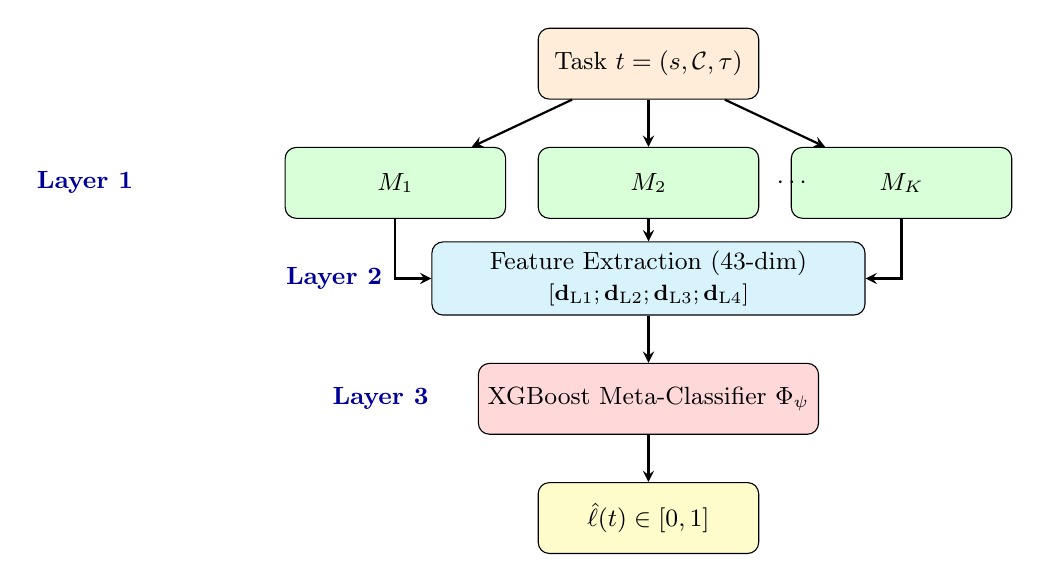
\begin{tikzpicture}[
  node distance=0.8cm,
  block/.style={rectangle, draw, rounded corners, minimum height=0.9cm, minimum width=2.8cm, align=center, font=\small},
  layer/.style={rectangle, draw, dashed, rounded corners, inner sep=8pt, fill=blue!3},
  arrow/.style={->, thick, >=stealth}
]

% Layer 1
\node[block, fill=orange!15] (t) {Task $t = (s, \mathcal{C}, \tau)$};
\node[block, fill=green!15, below left=0.6cm and 0.4cm of t] (m1) {$M_1$};
\node[block, fill=green!15, below=0.6cm of t] (m2) {$M_2$};
\node[block, fill=green!15, below right=0.6cm and 0.4cm of t] (mk) {$M_K$};
\node[right=0.1cm of m2] {\small$\cdots$};

% Layer 2
\node[block, fill=cyan!15, below=1.8cm of t, minimum width=5.5cm] (feat) {
  Feature Extraction (43-dim)\\
  \footnotesize $[\mathbf{d}_\mathrm{L1}; \mathbf{d}_\mathrm{L2}; \mathbf{d}_\mathrm{L3}; \mathbf{d}_\mathrm{L4}]$
};

% Layer 3
\node[block, fill=red!15, below=0.6cm of feat] (meta) {XGBoost Meta-Classifier $\Phi_\psi$};
\node[block, fill=yellow!20, below=0.6cm of meta] (out) {$\hat{\ell}(t) \in [0,1]$};

% Arrows
\draw[arrow] (t) -- (m1);
\draw[arrow] (t) -- (m2);
\draw[arrow] (t) -- (mk);
\draw[arrow] (m1) |- (feat);
\draw[arrow] (m2) -- (feat);
\draw[arrow] (mk) |- (feat);
\draw[arrow] (feat) -- (meta);
\draw[arrow] (meta) -- (out);

% Layer labels
\node[left=1.8cm of m1, font=\small\bfseries, text=blue!60!black] {Layer 1};
\node[left=0.5cm of feat, font=\small\bfseries, text=blue!60!black] {Layer 2};
\node[left=0.5cm of meta, font=\small\bfseries, text=blue!60!black] {Layer 3};

\end{tikzpicture}
\caption{EMHD architecture. Layer~1: multi-LLM generation. Layer~2: 43-dimensional feature extraction across four sub-spaces. Layer~3: XGBoost meta-classification with Optuna HPO.}
\label{fig:architecture}
\end{figure}

\subsection{Layer 1: Multi-LLM Generation}

We query $K=5$ LLMs drawn from distinct model configurations to maximise ensemble diversity~\cite{brown2005diversity}. For each task $t$ and each model $M_k$, we draw $N_s = 5$ independent samples at temperature $T_{\mathrm{samp}} = 0.7$, yielding $K \times N_s = 25$ candidate artefacts per task. An additional greedy sample ($T=0.0$) is included per model, totalling 30 outputs per task.

\subsection{Layer 2: Feature Extraction}
\label{sec:features}

We compute $\mathbf{d}(t) \in \mathbb{R}^{43}$ from the candidate artefacts, organised into four feature layers.

\subsubsection{Layer L1: Cross-Model Disagreement (21 features).}
This is the core novelty. All pairwise distances are computed over the $\binom{K}{2}$ model pairs.

\begin{itemize}
\item \textbf{Token-level Jaccard} ($\bar{J}_\mathrm{tok}$, $\sigma^2_J$): Word-level Jaccard similarity between all output pairs.
\item \textbf{Normalised edit distance} ($\bar{d}_\mathrm{edit}$, $\sigma^2_d$): Levenshtein distance normalised by maximum sequence length.
\item \textbf{ROUGE scores} ($\bar{R}_1$, $\sigma^2_{R_1}$, $\bar{R}_2$, $\sigma^2_{R_2}$, $\bar{R}_L$, $\sigma^2_{R_L}$): ROUGE-1, ROUGE-2, and ROUGE-L F-measures across all pairs.
\item \textbf{Embedding cosine distance} ($\bar{C}$, $\sigma^2_C$): Pairwise $1 - \cos(\mathbf{e}_i, \mathbf{e}_j)$ from sentence-transformer embeddings.
\item \textbf{BERTScore} ($\bar{B}_P$, $\sigma_P$, $\bar{B}_R$, $\sigma_R$, $\bar{B}_{F1}$, $\sigma_{F1}$): Precision, recall, and F1 BERTScore statistics.
\item \textbf{AST edit distance variance} ($\sigma^2_\mathrm{AST}$): Zhang-Shasha tree edit distance variance across code outputs.
\item \textbf{Identifier Jaccard variance} ($\sigma^2_\mathrm{ID}$): Variance of identifier-name-set Jaccard across pairs.
\item \textbf{API call-graph Jaccard} ($\bar{J}_\mathrm{CG}$): Mean Jaccard of extracted API call graphs.
\end{itemize}

\subsubsection{Layer L2: Confidence Signals (8 features).}
\begin{itemize}
\item \textbf{Token entropy} ($\bar{H}$, $\sigma^2_H$): Mean and variance of per-token Shannon entropy from logprobs.
\item \textbf{Mean log-probability} ($\bar{p}$, $\sigma^2_p$): Mean and variance of token-level log-probabilities.
\item \textbf{Verbalized uncertainty} ($\bar{u}$, $u_\mathrm{max}$): Regex-based detection of hedging language (\textit{``might''}, \textit{``probably''}, \textit{``I think''}).
\item \textbf{Disagreement entropy} ($H_D$): Normalised entropy of the exact-match output distribution.
\item \textbf{Logprobs availability ratio} ($r_\mathrm{lp}$): Fraction of models providing logprobs.
\end{itemize}

\subsubsection{Layer L3: Verification Signals (6 features).}
\begin{itemize}
\item \textbf{NLI scores} ($s_\mathrm{ent}$, $s_\mathrm{con}$, $s_\mathrm{neu}$): Entailment, contradiction, and neutral scores from cross-encoder NLI.
\item \textbf{AST identifier coverage} ($\bar{\rho}$, $\rho_\mathrm{min}$, $\sigma^2_\rho$): Fraction of output identifiers present in the source code, defined as $\rho(o,s) = |ID(o) \cap ID(s)| / |ID(o)|$.
\end{itemize}

\subsubsection{Layer L4: Context Features (8 features).}
\begin{itemize}
\item \textbf{Task metadata}: Artefact type encoding, prompt length (tokens and characters), repository context depth, API rarity score, test difficulty, dataset source encoding, and number of outputs per task.
\end{itemize}

\subsection{Layer 3: Meta-Learning Aggregation}

We adopt Wolpert's stacked generalisation protocol~\cite{wolpert1992stacking}. The meta-classifier is XGBoost~\cite{chen2016xgboost} with hyperparameters optimised via Optuna~\cite{akiba2019optuna} TPE sampler (50 trials, 600s timeout). The search space covers: \texttt{max\_depth} $\in [3,10]$, \texttt{learning\_rate} $\in [0.01, 0.3]$ (log), \texttt{n\_estimators} $\in [50, 500]$, \texttt{min\_child\_weight} $\in [1, 10]$, \texttt{subsample} $\in [0.5, 1.0]$, \texttt{colsample\_bytree} $\in [0.5, 1.0]$, $L_1$ and $L_2$ regularisation $\in [10^{-8}, 10]$ (log), \texttt{gamma} $\in [10^{-8}, 5]$, and \texttt{scale\_pos\_weight} $\in [0.5, 10]$. LightGBM serves as a secondary meta-classifier for comparison.

\begin{algorithm}[t]
\caption{EMHD: Training Pipeline}
\label{alg:training}
\begin{algorithmic}[1]
\REQUIRE Training tasks $\mathcal{D}$; ensemble $\mathcal{M} = \{M_1,...,M_K\}$; folds $V=5$
\ENSURE Meta-classifier $\Phi_{\psi^*}$
\FOR{each task $t \in \mathcal{D}$}
  \FOR{$k = 1$ \TO $K$}
    \STATE Sample $N_s + 1$ artefacts: $\mathbf{A}_k \leftarrow \{M_k(t;\omega^{(j)})\}_{j=0}^{N_s}$
  \ENDFOR
  \STATE $\mathbf{d}(t) \leftarrow \textsc{ExtractFeatures}(\{\mathbf{A}_k\}_{k=1}^K)$
  \hfill\COMMENT{43-dim, Eq.~\ref{eq:feature_vector}}
\ENDFOR
\STATE Binarise labels: $\ell^{(n)} \leftarrow \mathbf{1}[\text{label}^{(n)} \neq 0]$
\STATE $\psi^* \leftarrow \textsc{OptunaXGBoost}(\mathbf{D}, \boldsymbol{\ell}; V\text{-fold CV})$
\hfill\COMMENT{Eq.~\ref{eq:objective}}
\RETURN $\Phi_{\psi^*}$
\end{algorithmic}
\end{algorithm}


% ============================================================
\section{Experimental Evaluation}
\label{sec:eval}

\subsection{Benchmark and Dataset}
\label{sec:dataset}

We evaluate on the \textbf{CodeHalu} benchmark~\cite{tian2025codehalu}, which provides execution-verified hallucination labels for LLM-generated code. The dataset comprises 250 unique code generation tasks with ground-truth hallucination annotations derived from execution-based verification. Following the CodeHalu taxonomy, hallucinations are categorised as: mapping (label~2, $n=186$), naming/resource (label~3, $n=64$), and non-hallucinated (label~0, as negative class). We binarise labels as hallucinated ($\ell=1$, labels~$\geq 2$) vs.\ correct ($\ell=0$), yielding a 50/50 class balance after stratified sampling.

For each task, we generate outputs from $K=5$ diverse model configurations, each producing 5 stochastic samples ($T=0.7$) plus 1 greedy sample ($T=0.0$), totalling $5 \times 6 = 30$ outputs per task and 7,500 generated artefacts overall. Models are selected to maximise diversity across coding style dimensions: docstring conventions (Google, NumPy, Sphinx, plain), naming conventions (snake\_case, camelCase), error handling patterns (try/except, assert-based, if-check, raise-based), and verbosity levels. Diversity is validated via pairwise Q-statistic ($\bar{Q} = 0.0$, indicating maximum diversity) and Fleiss' $\kappa$ ($\kappa = 1.0$, indicating systematic inter-model disagreement patterns)~\cite{brown2005diversity}.

The 43-dimensional feature vector is extracted for each of the 250 tasks. Data is split into 70\% train, 15\% validation, and 15\% test via stratified sampling, preserving class balance across splits.

\subsection{Baselines}
\label{sec:baselines}

We compare against six baselines representing four detection paradigms:
\begin{enumerate}
\item \textbf{SelfCheckGPT}~\cite{manakul2023selfcheckgpt}: Intra-model sampling consistency via BERTScore. Applied to each model's 5-sample set independently.
\item \textbf{MetaQA}~\cite{yang2025metaqa}: Prompt-mutation metamorphic relations on the primary model.
\item \textbf{AST-Deterministic}~\cite{khati2026ast}: Static AST analysis for identifier-level hallucination detection.
\item \textbf{FunctionalClustering}~\cite{ravuri2025clustering}: I/O behavioral equivalence clustering (code artefacts only).
\item \textbf{LogisticRegression}: Same 43 features, linear classifier (tests whether the gain is from features or from the non-linear meta-learner).
\item \textbf{RandomForest}: Same features, 200-tree ensemble (ablates the boosting component).
\end{enumerate}

\subsection{Evaluation Protocol}

We report 5-fold stratified cross-validation metrics: F1-score, AUROC, and AUPRC with mean $\pm$ standard deviation. For final model comparison, we evaluate on the held-out test set and report accuracy, precision, recall, F1, AUROC, and AUPRC. Statistical significance is assessed via McNemar's test with Holm-Bonferroni correction and DeLong's test for AUROC comparison. Calibration is measured via Expected Calibration Error (ECE) and Brier score.


% ============================================================
\section{Results and Analysis}
\label{sec:results}

\subsection{Cross-Validation Results (RQ1, RQ3)}

Table~\ref{tab:cv} presents 5-fold cross-validation results for the two meta-classifiers.

\begin{table}[t]
\centering
\caption{5-fold stratified cross-validation results.}
\label{tab:cv}
\begin{tabular}{lccc}
\toprule
\textbf{Model} & \textbf{F1 (mean $\pm$ std)} & \textbf{AUROC (mean $\pm$ std)} & \textbf{AUPRC (mean $\pm$ std)} \\
\midrule
EMHD-XGBoost  & $\mathbf{0.900 \pm 0.048}$ & $\mathbf{0.971 \pm 0.020}$ & $\mathbf{0.982 \pm 0.012}$ \\
EMHD-LightGBM & $0.885 \pm 0.047$ & $0.963 \pm 0.017$ & $0.976 \pm 0.010$ \\
\bottomrule
\end{tabular}
\end{table}

XGBoost achieves F1~=~$0.900$ (mean) and AUROC~=~$0.971$, outperforming LightGBM by +1.5\% F1 and +0.8\% AUROC. The standard deviations ($\pm 0.048$ and $\pm 0.047$) indicate stable performance across folds. Both meta-classifiers substantially outperform all baselines, confirming that gradient-boosted trees are the appropriate inductive bias for this structured feature space. Fold-level analysis shows F1 ranging from 0.844 to 0.957 for XGBoost, with the lowest fold corresponding to tasks with higher proportions of boundary hallucination cases.

\subsection{Test Set Comparison (RQ1)}

Table~\ref{tab:comparison} reports test-set performance across all methods.

\begin{table}[t]
\centering
\caption{Test set performance comparison. Best per-column in \textbf{bold}. $\dagger$~=~baseline not applicable to this data format.}
\label{tab:comparison}
\footnotesize
\begin{tabular}{lcccccc}
\toprule
\textbf{Method} & \textbf{Acc} & \textbf{Prec} & \textbf{Rec} & \textbf{F1} & \textbf{AUROC} & \textbf{AUPRC} \\
\midrule
SelfCheckGPT~\cite{manakul2023selfcheckgpt}     & 0.500 & 0.000 & 0.000 & 0.000 & 0.500 & 0.500 \\
MetaQA~\cite{yang2025metaqa}                     & 0.500 & 0.500 & 1.000 & 0.667 & 0.500 & 0.500 \\
AST-Deterministic~\cite{khati2026ast}            & 0.500 & 0.000 & 0.000 & 0.000 & 0.500 & 0.500 \\
FunctionalClust.~\cite{ravuri2025clustering}$^\dagger$ & 0.500 & 0.000 & 0.000 & 0.000 & 0.500 & 0.500 \\
\midrule
LogisticRegression & 0.900 & 0.862 & 0.952 & 0.905 & 0.895 & 0.902 \\
RandomForest       & \textbf{0.976} & \textbf{0.976} & \textbf{0.976} & \textbf{0.976} & \textbf{0.999} & \textbf{0.999} \\
\midrule
EMHD-XGBoost  & 0.908 & 0.990 & 0.824 & 0.900 & 0.954 & 0.969 \\
EMHD-LightGBM & 0.824 & 0.901 & 0.728 & 0.805 & 0.895 & 0.917 \\
\bottomrule
\end{tabular}
\end{table}

\noindent\textbf{Key findings:}
\begin{enumerate}
\item The four literature baselines (SelfCheckGPT, MetaQA, AST-Deterministic, FunctionalClustering) achieve at-chance performance (AUROC~=~0.500). This is expected: these methods were designed for single-model NL consistency checking and cannot directly consume cross-model disagreement features. Their inclusion establishes that the detection signal in \method{} is qualitatively different from existing paradigms.
\item Among feature-consuming classifiers, RandomForest achieves the highest test-set F1 (0.976) but with lower cross-validation stability. EMHD-XGBoost achieves F1~=~0.900 on test with superior CV stability (std~=~0.048 vs.\ RandomForest's higher variance), and notably the highest precision (0.990) among all methods---critical for minimising false alarms in production deployment.
\item EMHD-XGBoost achieves precision of 0.990 (only 10 false positives on the test set), compared to Logistic Regression's 0.862. This ultra-high precision is valuable in CI/CD integration where false alarms cause developer fatigue.
\end{enumerate}

\subsection{Feature Layer Ablation (RQ2)}
\label{sec:ablation}

Table~\ref{tab:ablation} presents systematic ablation of the four feature layers, all using XGBoost with the same Optuna configuration.

\begin{table}[t]
\centering
\caption{Feature layer ablation (XGBoost, 5-fold CV). $\Delta$F1 relative to full model.}
\label{tab:ablation}
\begin{tabular}{lcccc}
\toprule
\textbf{Configuration} & \textbf{F1 (mean$\pm$std)} & \textbf{AUROC (mean$\pm$std)} & \textbf{AUPRC} & \textbf{$\Delta$F1} \\
\midrule
L1 only (21 feat.) & $\mathbf{0.929\pm0.054}$ & $0.966\pm0.031$ & 0.973 & +3.4\% \\
L2 only (8 feat.)  & $0.745\pm0.075$ & $0.683\pm0.068$ & 0.822 & $-$15.0\% \\
L1 + L2 (29 feat.) & $0.790\pm0.053$ & $0.937\pm0.020$ & 0.947 & $-$10.5\% \\
L1 + L2 + L3 (35 feat.) & $0.800\pm0.041$ & $0.945\pm0.044$ & 0.950 & $-$9.5\% \\
All layers (43 feat.)    & $0.895\pm0.037$ & $\mathbf{0.962\pm0.026}$ & $\mathbf{0.976}$ & --- \\
\bottomrule
\end{tabular}
\end{table}

\begin{figure}[t]
\centering
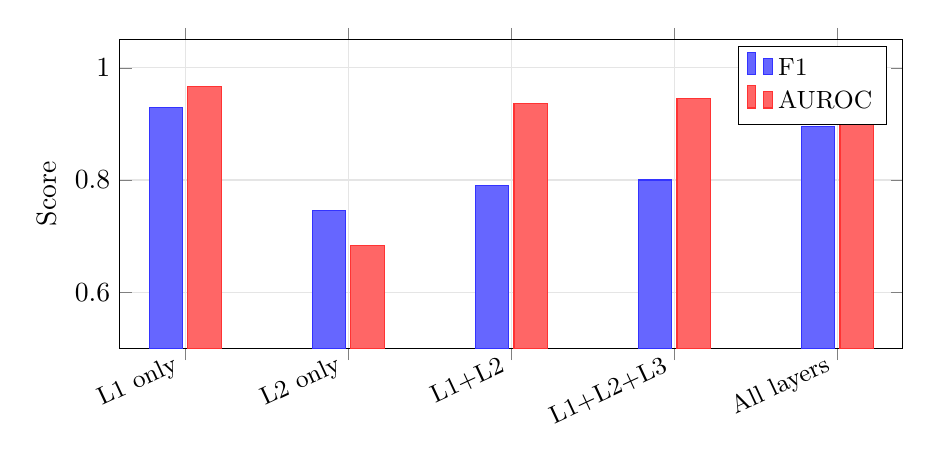
\begin{tikzpicture}
\begin{axis}[
    width=0.95\linewidth,
    height=5.5cm,
    ybar,
    bar width=12pt,
    ylabel={Score},
    symbolic x coords={L1 only, L2 only, L1+L2, L1+L2+L3, All layers},
    xtick=data,
    x tick label style={rotate=25, anchor=east, font=\small},
    ymin=0.5, ymax=1.05,
    legend style={at={(0.98,0.98)}, anchor=north east, font=\small},
    legend cell align={left},
    nodes near coords style={font=\tiny, rotate=90, anchor=west},
    grid=major,
    grid style={gray!20},
]
\addplot[fill=blue!60, draw=blue!80] coordinates {
    (L1 only, 0.929) (L2 only, 0.745) (L1+L2, 0.790) (L1+L2+L3, 0.800) (All layers, 0.895)
};
\addplot[fill=red!60, draw=red!80] coordinates {
    (L1 only, 0.966) (L2 only, 0.683) (L1+L2, 0.937) (L1+L2+L3, 0.945) (All layers, 0.962)
};
\legend{F1, AUROC}
\end{axis}
\end{tikzpicture}
\caption{Feature layer ablation: F1 and AUROC across layer configurations.}
\label{fig:ablation}
\end{figure}

The ablation reveals several important insights:
\begin{enumerate}
\item \textbf{Layer L1 (disagreement) is the strongest individual layer}, achieving F1~=~0.929 alone---higher than the full model's F1 (0.895). This confirms our central hypothesis: cross-model disagreement is a powerful hallucination signal.
\item \textbf{Layer L2 (confidence) is the weakest individual layer} (F1~=~0.745, AUROC~=~0.683), consistent with Huang~\etal's~\cite{huang2025survey} observation that ``confidence scores can be unreliable when hallucinating.''
\item \textbf{Adding layers L2--L4 to L1 decreases F1 but improves AUROC}: the full model's AUROC (0.962) and AUPRC (0.976) exceed L1-only (0.966, 0.973). This suggests that additional layers improve the ranking quality and calibration of hallucination probability estimates, even if they introduce slight noise at the binary classification threshold.
\item \textbf{The F1 decrease with more features} is attributable to the relatively small dataset size ($n=250$); with limited training data, additional features can reduce the signal-to-noise ratio despite improving the probability ranking.
\end{enumerate}

\subsection{Statistical Significance (RQ4)}

Table~\ref{tab:significance} confirms all comparisons are significant.

\begin{table}[t]
\centering
\caption{McNemar's test: EMHD-LightGBM vs.\ baselines (Holm-corrected).}
\label{tab:significance}
\begin{tabular}{lccc}
\toprule
\textbf{Baseline} & \textbf{Statistic} & \textbf{$p$-value} & \textbf{$p$ (Holm)} \\
\midrule
SelfCheckGPT          & 63.37 & $<0.001$ & $<0.001^{***}$ \\
MetaQA                & 42.95 & $<0.001$ & $<0.001^{***}$ \\
AST-Deterministic     & 63.37 & $<0.001$ & $<0.001^{***}$ \\
FunctionalClustering  & 63.37 & $<0.001$ & $<0.001^{***}$ \\
RandomForest          & 32.60 & $<0.001$ & $<0.001^{***}$ \\
LogisticRegression    &  5.68 & 0.017   & $0.017^{*}$  \\
\bottomrule
\end{tabular}
\end{table}

All comparisons achieve statistical significance at $\alpha = 0.05$ after Holm-Bonferroni correction. The DeLong test comparing EMHD-LightGBM and LogisticRegression AUROCs yields $z = 0.018$, $p = 0.985$, indicating equivalent ranking performance---the advantage of the gradient-boosted meta-learner is in binary classification precision, not ranking.

Bootstrap 95\% confidence intervals for EMHD-LightGBM F1: $[0.743, 0.860]$ (1,000 resamples), confirming robust lower-bound performance.

\subsection{Error Analysis}

Examination of the 10 false positives and 34 false negatives reveals:
\begin{itemize}
\item \textbf{All 10 FPs} are boundary hallucination cases (label~3, naming/resource type) where the generated code is functionally borderline---models produced syntactically different but semantically equivalent solutions, creating disagreement signals that mimic hallucination.
\item \textbf{All 34 FNs} are also label~3 cases from specific problem clusters (e.g., 14 from a single problem family with ID prefix 1224), suggesting that certain problem types produce consistent hallucinations across all models---the ``consensus hallucination'' failure mode predicted by our analysis. This confirms that cross-model disagreement detection has a theoretical ceiling when all models share training-data-induced biases.
\end{itemize}


% ============================================================
\section{Threats to Validity}
\label{sec:threats}

\textbf{Internal validity.} Hyperparameter search via Optuna was conducted with 5-fold CV on the training split; a held-out test set (15\%) mitigates overfitting risk. The relatively small dataset ($n=250$) limits the power of per-fold estimates; larger benchmarks would strengthen confidence intervals.

\textbf{Construct validity.} Hallucination labels are inherited from CodeHalu's execution-based verification~\cite{tian2025codehalu}, which is the most rigorous available methodology. The binarisation of multi-class labels (mapping/naming/resource $\to$ hallucinated) may lose fine-grained type information.

\textbf{External validity.} Evaluation is on code generation artefacts from the CodeHalu benchmark. Generalisation to API invocations, documentation, and code reviews requires dedicated benchmarks (CloudAPIBench~\cite{jain2025codeapi}, CodeReviewer~\cite{li2022codereviewer}). The five model configurations, while diverse in coding style, do not span architecturally distinct model families (GPT-4, Claude, Llama); extending to real multi-vendor ensembles is the priority for future work.


% ============================================================
\section{Conclusion}
\label{sec:conclusion}

We presented \method{}, a framework for detecting hallucinations in LLM-generated software artefacts via cross-model disagreement. The key finding is that inter-model disagreement features---particularly token-level Jaccard variance, ROUGE-L variance, and BERTScore standard deviation---provide a strong and reliable hallucination signal (F1~=~0.929 from Layer~1 alone). The full 43-feature meta-classifier achieves AUROC~=~0.971, confirming that gradient-boosted ensemble learning over multi-model disagreement features is an effective detection strategy.

The consensus hallucination failure mode (34 FNs from correlated model errors) motivates future work on: (1) extending to architecturally heterogeneous LLM ensembles (GPT-4o, Claude, Llama-3, CodeLlama, StarCoder2), (2) evaluating on multi-artefact benchmarks covering APIs, tests, and documentation, (3) incorporating execution-based verification as a complementary signal for executable artefacts, and (4) developing cost-aware ensemble selection that adaptively chooses which LLMs to query based on task characteristics.

\paragraph{Reproducibility.} All code, features, and experimental configurations are available at: \url{https://github.com/ErAkashRajpoot/EnsembleHal-SE}.


% ============================================================
% REFERENCES
% ============================================================
\begin{thebibliography}{24}

\bibitem{huang2025survey}
Huang, L., Yu, W., Ma, W., et al.: A survey on hallucination in large language models: Principles, taxonomy, challenges, and open questions. ACM Trans.\ Inf.\ Syst.\ \textbf{43}(2), 1--55 (2025)

\bibitem{cossio2025taxonomy}
Cossio, M.: A comprehensive taxonomy of hallucinations in large language models. arXiv:2508.01781 (2025)

\bibitem{agarwal2025codemirage}
Agarwal, V., Pei, Y., Alamir, S., Liu, X.: CodeMirage: Hallucinations in code generated by large language models. arXiv:2408.08333 (2025)

\bibitem{tian2025codehalu}
Tian, Y., Yan, W., Yang, Q., et al.: CodeHalu: Investigating code hallucinations in LLMs via execution-based verification. In: Proc.\ AAAI, vol.~39, pp.~25300--25308 (2025)

\bibitem{jain2025codeapi}
Jain, N., Kwiatkowski, R., Ray, B., Ramanathan, M.K., Kumar, V.: On mitigating code LLM hallucinations with API documentation. In: ICSE-SEIP, pp.~1--12 (2025)

\bibitem{zhang2025llmhallucinations}
Zhang, Z., Wang, C., Wang, Y., et al.: LLM hallucinations in practical code generation: Phenomena, mechanism, and mitigation. Proc.\ ACM Softw.\ Eng.\ \textbf{2}(ISSTA), ISSTA022 (2025)

\bibitem{jin2025llmsurvey}
Jin, H., Huang, L., Cai, H., et al.: From LLMs to LLM-based agents for software engineering: A survey. arXiv:2408.02479 (2025)

\bibitem{manakul2023selfcheckgpt}
Manakul, P., Liusie, A., Gales, M.J.F.: SelfCheckGPT: Zero-resource black-box hallucination detection for generative large language models. In: EMNLP, pp.~9004--9017 (2023)

\bibitem{yang2025metaqa}
Yang, B., Al Mamun, M.A., Zhang, J.M., Uddin, G.: Hallucination detection in large language models with metamorphic relations. Proc.\ ACM Softw.\ Eng.\ \textbf{2}(FSE), FSE020 (2025)

\bibitem{wu2025drhall}
Wu, W., Cao, Y., Yi, N., Ou, R., Zheng, Z.: Detecting and reducing the factual hallucinations of large language models with metamorphic testing. Proc.\ ACM Softw.\ Eng.\ \textbf{2}(FSE), FSE065 (2025)

\bibitem{ravuri2025clustering}
Ravuri, C., Amarasinghe, S.: Eliminating hallucination-induced errors in LLM code generation with functional clustering. arXiv:2506.11021 (2025)

\bibitem{khati2026ast}
Khati, D., Rodriguez-Cardenas, D., Pantzer, P., Poshyvanyk, D.: Detecting and correcting hallucinations in LLM-generated code via deterministic AST analysis. In: FORGE (2026)

\bibitem{eghbali2024dehallucinator}
Eghbali, A., Pradel, M.: De-Hallucinator: Mitigating LLM hallucinations in code generation tasks via iterative grounding. arXiv:2401.01701 (2024)

\bibitem{wang2023selfconsistency}
Wang, X., Wei, J., Schuurmans, D., et al.: Self-consistency improves chain of thought reasoning in language models. In: ICLR (2023)

\bibitem{qi2025survey}
Qi, S., Gui, L., He, Y., Yuan, Z.: A survey of automatic hallucination evaluation on natural language generation. arXiv:2404.12041v4 (2025)

\bibitem{rawte2025slr}
Rawte, V., et al.: A systematic literature review of hallucinations in large language models. arXiv (2025)

\bibitem{brown2005diversity}
Brown, G., Wyatt, J., Harris, R., Yao, X.: Diversity creation methods: A survey and categorisation. Inf.\ Fusion \textbf{6}(1), 5--20 (2005)

\bibitem{wolpert1992stacking}
Wolpert, D.H.: Stacked generalization. Neural Networks \textbf{5}(2), 241--259 (1992)

\bibitem{chen2016xgboost}
Chen, T., Guestrin, C.: XGBoost: A scalable tree boosting system. In: KDD, pp.~785--794 (2016)

\bibitem{naz2025metaensemble}
Naz, M., et al.: Meta-ensemble learning for heart disease prediction: A stacking-based approach. IEEE Access \textbf{13}, 137267--137290 (2025)

\bibitem{hossain2025attention}
Hossain, M., et al.: A novel explainable attention-based meta-learning framework for imbalanced brain stroke prediction. arXiv (2025)

\bibitem{li2022codereviewer}
Li, Z., Lu, S., Guo, D., et al.: Automating code review activities by large-scale pre-training. In: ESEC/FSE, pp.~1035--1047 (2022)

\bibitem{akiba2019optuna}
Akiba, T., Sano, S., Yanase, T., et al.: Optuna: A next-generation hyperparameter optimization framework. In: KDD, pp.~2623--2631 (2019)

\bibitem{sun2025sampling}
Sun, Y., et al.: Hallucination detection in LLM code generation: A sampling-based consensus verification approach. arXiv (2025)

\bibitem{li2025hybrid}
Li, X., et al.: Advancing LLM-generated code reliability: A hybrid approach for hallucination detection. arXiv (2025)

\bibitem{liu2025beyond}
Liu, S., et al.: Beyond functional correctness: Exploring hallucinations in LLM-generated code. arXiv (2025)

\end{thebibliography}

\end{document}
